\section{\textbf{Resultados}}

\subsection{\textbf{Fuente \textit{S}}}

\begin{center}\small
	\begin{tabular}{ c | c | c | c | c }
	   & ComercioLibre & CoinFactory & Café & Cumpleaños \\ \hline
	  \textit{I}($\SimbBroadcast$) & 5.13 & 4.54 & 0.00577 & 0.53 \\ 
	  \textit{I}($\SimbUnicast$) & 0.04 & 0.06 & 0.994 & 1.68 \\ 
	  \textit{H(S)} & 0.187 & 0.256 & 0.051 & 0.894 \\ 
	  $N$ &  & 47 & aa & 26 \\ 
	  $M$ & 14675 & 12621 & 77274 & 3812 \\
	\end{tabular}
\end{center}

Donde $N$ es la cantidad de nodos identificados y $M$ la de mensajes leídos durante la captura. Consideramos como conjunto de \textit{nodos} al conjunto de \textit{MACs} de origen distintas.

Suponiendo que los nodos en las redes se comportan de manera similar, los datos sugieren que cuantos más nodos hay en la red la probabilidad de \textit{S} de emitir $\SimbBroadcast$ disminuye y la información que este símbolo aporta aumenta. En cambio, una menor cantidad de nodos aproxima su entropía a su máximo valor, o lo que es igual, asemeja las probabilidades de ambos símbolos.

\subsection{\textbf{Fuente \textit{S}$_1$}}

\subsection*{\textbf{ComercioLibre}}

\begin{center}\small
	\begin{tabular}{ c | c | c | c }
	  \textit{H(S$_1$)} & \textit{Max H(S$_1$)} & \textbar \textit{distinguidos}\textbar & \textbar Nodos\textbar \\
	  \hline
	  3.60 & 6 & 2 & 67 \\
	\end{tabular}
\end{center}
Donde los símbolos \textit{distinguidos} son \{10.10.35.10, 10.10.34.241\}.

\begin{figure}[htb]
	\centering
	% Por si tenemos problemas y necesitamos achicarlo esto sirve sin romper IEEE
	%\resizebox{2cm}{!}{\begin{tikzpicture}
    \tikzset{NoDistinguido/.style = {shape=circle,draw,thick,minimum size=2em,font=\tiny}}
    \tikzset{Distinguido/.style = {shape=circle,draw,red,thick,minimum size=2em,font=\scriptsize}}
    \tikzset{myCloud/.style = {shape=cloud,draw, cloud puffs=10,cloud puff arc=110, aspect=2, inner ysep=0.5em}}

    \tikzset{flecha/.style = {->,>=stealth,black,sloped,auto=false}}

    \node[myCloud] (NubeA) at (-2,2) {8 vértices};
    \node[myCloud] (NubeB) at (-2,4) {2 vértices};

    \node[myCloud] (NubeC) at (1,3) {2 vértices};

    \node[NoDistinguido] (aparenteRouter) at (0,0) {10.10.35.1};
    \node[NoDistinguido] (node66) at (2,0) {10.10.35.66};


    \node[NoDistinguido] (node0) at (-2,0.5) {0.0.0.0};
    \node[Distinguido] (dist1) at (-2,-2) {10.10.35.10};
    \node[NoDistinguido] (node255) at (-2,-4.5) {169.254.255.255};
    \node[NoDistinguido] (node223) at (0,-6) {10.10.35.223};

    \node[Distinguido] (dist2) at (1,-3) {10.10.35.241};


    %Entradas a la nubeA
    \draw [flecha] (aparenteRouter) to node[above] {10} (NubeA);
    \draw [flecha] (NubeB) to node[above] {2} (NubeA);

    %Aparente router a vértices Distinguidos
    \draw [flecha] (aparenteRouter) to node[above] {12} (dist1);
    \draw [flecha] (aparenteRouter) to node[above] {52} (dist2);

    %Un colgado
    \draw [flecha] (node66) to node[above] {3} (aparenteRouter);

    %

    \draw [flecha] (node0) to node[above] {3} (dist1);

    \draw [flecha] (dist1) to node[above] {14} (node255);
    \path[flecha] (dist1)
            edge [loop right=30] node [above] {7} ();

    \draw [flecha] (node223) to node[above] {5} (node255);
    \path[flecha] (node223)
            edge [loop right=30] node [above] {2} ();


    \draw [flecha] (NubeC) to node[above] {7} (aparenteRouter);
    \path[flecha] (NubeC)
            edge [loop left] node [above] {12} ();

%\iffalse
%Dejo esto por si quieren partir la Nube C
%    \node[NoDistinguido] (node37) at (0,2) {10.10.35.37};
%    \node[NoDistinguido] (node141) at (2,2) {10.10.35.141};
%    \draw [flecha] (node37) to node[above] {3} (aparenteRouter);
%    \path[flecha] (node37)
%            edge [loop above] node [above] {6} ();
%
%    \draw [flecha] (node141) to node[above] {4} (aparenteRouter);
%    \path[flecha] (node141)
%            edge [loop right=30] node [above] {6} ();
%\fi

\end{tikzpicture}
}
	\begin{tikzpicture}
    \tikzset{NoDistinguido/.style = {shape=circle,draw,thick,minimum size=2em,font=\tiny}}
    \tikzset{Distinguido/.style = {shape=circle,draw,red,thick,minimum size=2em,font=\scriptsize}}
    \tikzset{myCloud/.style = {shape=cloud,draw, cloud puffs=10,cloud puff arc=110, aspect=2, inner ysep=0.5em}}

    \tikzset{flecha/.style = {->,>=stealth,black,sloped,auto=false}}

    \node[myCloud] (NubeA) at (-2,2) {8 vértices};
    \node[myCloud] (NubeB) at (-2,4) {2 vértices};

    \node[myCloud] (NubeC) at (1,3) {2 vértices};

    \node[NoDistinguido] (aparenteRouter) at (0,0) {10.10.35.1};
    \node[NoDistinguido] (node66) at (2,0) {10.10.35.66};


    \node[NoDistinguido] (node0) at (-2,0.5) {0.0.0.0};
    \node[Distinguido] (dist1) at (-2,-2) {10.10.35.10};
    \node[NoDistinguido] (node255) at (-2,-4.5) {169.254.255.255};
    \node[NoDistinguido] (node223) at (0,-6) {10.10.35.223};

    \node[Distinguido] (dist2) at (1,-3) {10.10.35.241};


    %Entradas a la nubeA
    \draw [flecha] (aparenteRouter) to node[above] {10} (NubeA);
    \draw [flecha] (NubeB) to node[above] {2} (NubeA);

    %Aparente router a vértices Distinguidos
    \draw [flecha] (aparenteRouter) to node[above] {12} (dist1);
    \draw [flecha] (aparenteRouter) to node[above] {52} (dist2);

    %Un colgado
    \draw [flecha] (node66) to node[above] {3} (aparenteRouter);

    %

    \draw [flecha] (node0) to node[above] {3} (dist1);

    \draw [flecha] (dist1) to node[above] {14} (node255);
    \path[flecha] (dist1)
            edge [loop right=30] node [above] {7} ();

    \draw [flecha] (node223) to node[above] {5} (node255);
    \path[flecha] (node223)
            edge [loop right=30] node [above] {2} ();


    \draw [flecha] (NubeC) to node[above] {7} (aparenteRouter);
    \path[flecha] (NubeC)
            edge [loop left] node [above] {12} ();

%\iffalse
%Dejo esto por si quieren partir la Nube C
%    \node[NoDistinguido] (node37) at (0,2) {10.10.35.37};
%    \node[NoDistinguido] (node141) at (2,2) {10.10.35.141};
%    \draw [flecha] (node37) to node[above] {3} (aparenteRouter);
%    \path[flecha] (node37)
%            edge [loop above] node [above] {6} ();
%
%    \draw [flecha] (node141) to node[above] {4} (aparenteRouter);
%    \path[flecha] (node141)
%            edge [loop right=30] node [above] {6} ();
%\fi

\end{tikzpicture}

\end{figure}


\begin{figure}
  \begin{center}
    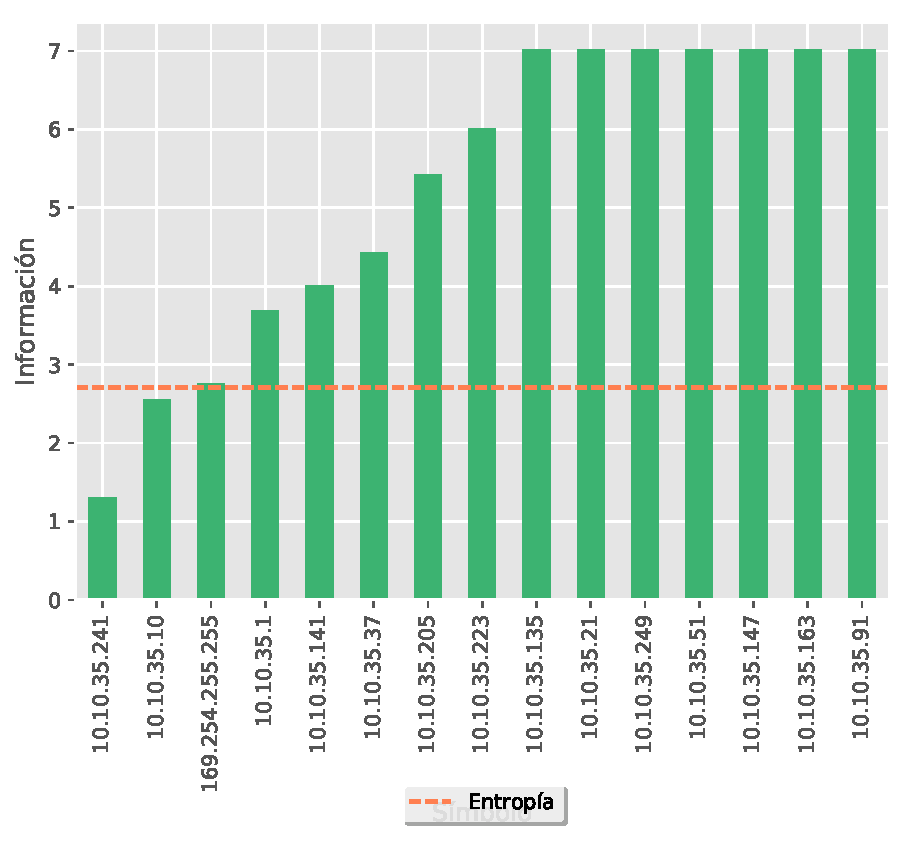
\includegraphics[scale = 0.5]{img/ECommerce-information-S1.pdf}
    \caption{Información de los simbolos de la fuente S1 para ComercioLibre}
    \label{informacion_ecommerce}
  \end{center}
\end{figure}

\subsection*{\textbf{CoinFactory}}

\begin{center}\small
	\begin{tabular}{ c | c | c | c }
	  \textit{H(S$_1$)} & \textit{Max H(S$_1$)} & \textbar \textit{distinguidos}\textbar & \textbar Nodos\textbar \\
	  \hline
	  1.90 & 3.91 & 1 & 15 \\
	\end{tabular}
\end{center}
Donde el símbolo \textit{distinguido} es \{192.168.0.129\}.

\begin{figure}[htb]
	\centering
	% Por si tenemos problemas y necesitamos achicarlo esto sirve sin romper IEEE
	%\resizebox{2cm}{!}{\begin{tikzpicture}

    \tikzset{vertex/.style = {shape=circle,draw,thick,minimum size=2em,font=\tiny}}
    \tikzset{NoDistinguido/.style = {shape=circle,draw,thick,minimum size=2em,font=\tiny}}
    \tikzset{Distinguido/.style = {shape=circle,draw,red,thick,minimum size=2em,font=\scriptsize}}
    \tikzset{myCloud/.style = {shape=cloud,draw, cloud puffs=10,cloud puff arc=110, aspect=2, inner ysep=0.5em}}

    \tikzset{myCloudSmaller/.style = {shape=cloud,draw, cloud puffs=9,cloud puff arc=110, aspect=3, inner ysep=0em, inner xsep=0em}}
    \tikzset{flecha/.style = {->,>=stealth,sloped,auto=false}}

    \node [NoDistinguido] (router1) at (3,0) {192.168.0.1};
    \node [Distinguido] (nodo129) at (3,5) {192.168.0.129};
    \draw [flecha] (router1)
        to node[above] {354} (nodo129);


    \node [NoDistinguido] (router2) at (-3,1) {192.168.0.2};


    %IPs 173, 163
    \node [myCloudSmaller] (NubeE) at (0,6) {2 vértices};
    \draw [flecha] (router2)
        to node[above] {3} (NubeE);
    \draw [flecha] (NubeE)
        to node[above] {29} (router1);


    %IPS 114, 118,  121, 122,  123, 145, 164, 178
    \node [myCloud] (NubeA) at (1,-1.5) {6 vértices};
    \draw [flecha] (NubeA)
        to node[above] {19} (router1);
    \draw [flecha] (NubeA)
        to [bend left=10] node[above] {17} (router2);
    \draw [flecha] (router2)
        to [bend left=10] node[above] {2} (NubeA);


    %IPs 177, 153 y 168
    \node [myCloudSmaller] (NubeB) at (0.5,-4) {3 vértices};
    \draw [flecha] (NubeB)
            to[bend left=5] node[above] {13} (router2);


    \node [myCloudSmaller] (NubeF) at (2.5,-4) {2 vértices};
    \draw [flecha] (NubeF)
         to node[above] {3} (router1);
    \draw [flecha] (NubeF)
         to[bend left=5] node[above] {7} (router2);
    \draw [flecha] (NubeF)
        to node[above] {3} (NubeA);
    \path[->,flecha] (NubeF)
            edge [loop below] node [above] {3} ();


    %IPs 102, 116, 139 y 154
    \node [myCloud] (NubeC) at (1,-7) {4 vértices};
    \draw [flecha] (router2)
        to node[above] {2} (NubeC);
    \draw [flecha] (NubeF)
        to node[above] {14} (NubeC);


    %IPs 109, 137
    \node[myCloudSmaller] (NubeD) at (-3,4) {2 vértices};
    \draw [flecha] (NubeD)
        to [bend left=5] node[above] {3} (router1);
    \draw [flecha] (NubeD)
        to node[above] {6} (router2);
    \draw [flecha] (NubeD)
        to node[above] {2} (NubeE);


    \node [NoDistinguido] (nodo149) at (0,1) {192.168.0.149};
    \draw [flecha] (nodo149)
        to node[above] {8} (NubeE);
    \draw [flecha] (nodo149)
        to [bend right=15]  node[above] {8} (router2);
    \draw [flecha] (router2)
        to [bend right=15]  node[above] {8} (nodo149);
    \draw [flecha] (router1)
        to node[above] {41} (nodo149);


    \node [NoDistinguido] (nodo167) at (-2,-4) {192.168.0.167};
    \draw [flecha] (router2)
        to node[above] {1} (nodo167);
    \path[->,flecha] (nodo167)
            edge [loop below] node [above] {6} ();

\end{tikzpicture}
}
	\begin{tikzpicture}

    \tikzset{vertex/.style = {shape=circle,draw,thick,minimum size=2em,font=\tiny}}
    \tikzset{NoDistinguido/.style = {shape=circle,draw,thick,minimum size=2em,font=\tiny}}
    \tikzset{Distinguido/.style = {shape=circle,draw,red,thick,minimum size=2em,font=\scriptsize}}
    \tikzset{myCloud/.style = {shape=cloud,draw, cloud puffs=10,cloud puff arc=110, aspect=2, inner ysep=0.5em}}

    \tikzset{myCloudSmaller/.style = {shape=cloud,draw, cloud puffs=9,cloud puff arc=110, aspect=3, inner ysep=0em, inner xsep=0em}}
    \tikzset{flecha/.style = {->,>=stealth,sloped,auto=false}}

    \node [NoDistinguido] (router1) at (3,0) {192.168.0.1};
    \node [Distinguido] (nodo129) at (3,5) {192.168.0.129};
    \draw [flecha] (router1)
        to node[above] {354} (nodo129);


    \node [NoDistinguido] (router2) at (-3,1) {192.168.0.2};


    %IPs 173, 163
    \node [myCloudSmaller] (NubeE) at (0,6) {2 vértices};
    \draw [flecha] (router2)
        to node[above] {3} (NubeE);
    \draw [flecha] (NubeE)
        to node[above] {29} (router1);


    %IPS 114, 118,  121, 122,  123, 145, 164, 178
    \node [myCloud] (NubeA) at (1,-1.5) {6 vértices};
    \draw [flecha] (NubeA)
        to node[above] {19} (router1);
    \draw [flecha] (NubeA)
        to [bend left=10] node[above] {17} (router2);
    \draw [flecha] (router2)
        to [bend left=10] node[above] {2} (NubeA);


    %IPs 177, 153 y 168
    \node [myCloudSmaller] (NubeB) at (0.5,-4) {3 vértices};
    \draw [flecha] (NubeB)
            to[bend left=5] node[above] {13} (router2);


    \node [myCloudSmaller] (NubeF) at (2.5,-4) {2 vértices};
    \draw [flecha] (NubeF)
         to node[above] {3} (router1);
    \draw [flecha] (NubeF)
         to[bend left=5] node[above] {7} (router2);
    \draw [flecha] (NubeF)
        to node[above] {3} (NubeA);
    \path[->,flecha] (NubeF)
            edge [loop below] node [above] {3} ();


    %IPs 102, 116, 139 y 154
    \node [myCloud] (NubeC) at (1,-7) {4 vértices};
    \draw [flecha] (router2)
        to node[above] {2} (NubeC);
    \draw [flecha] (NubeF)
        to node[above] {14} (NubeC);


    %IPs 109, 137
    \node[myCloudSmaller] (NubeD) at (-3,4) {2 vértices};
    \draw [flecha] (NubeD)
        to [bend left=5] node[above] {3} (router1);
    \draw [flecha] (NubeD)
        to node[above] {6} (router2);
    \draw [flecha] (NubeD)
        to node[above] {2} (NubeE);


    \node [NoDistinguido] (nodo149) at (0,1) {192.168.0.149};
    \draw [flecha] (nodo149)
        to node[above] {8} (NubeE);
    \draw [flecha] (nodo149)
        to [bend right=15]  node[above] {8} (router2);
    \draw [flecha] (router2)
        to [bend right=15]  node[above] {8} (nodo149);
    \draw [flecha] (router1)
        to node[above] {41} (nodo149);


    \node [NoDistinguido] (nodo167) at (-2,-4) {192.168.0.167};
    \draw [flecha] (router2)
        to node[above] {1} (nodo167);
    \path[->,flecha] (nodo167)
            edge [loop below] node [above] {6} ();

\end{tikzpicture}

\end{figure}

\begin{figure}
  \begin{center}
    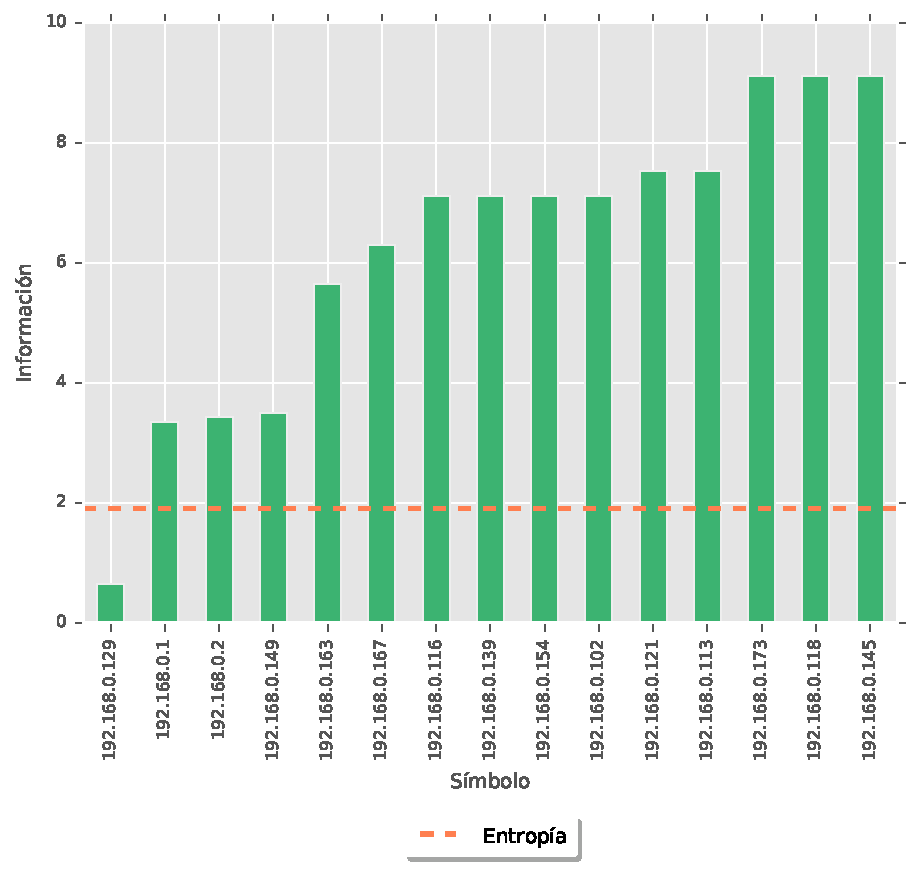
\includegraphics[scale = 0.5]{img/Pyme-information-S1.pdf}
    \caption{Información de los simbolos de la fuente S1 para CoinFactory}
    \label{informacion_pyme}
  \end{center}
\end{figure}

\subsection*{\textbf{Café}}

% \begin{center}\small
% 	\begin{tabular}{ c | c | c | c }
% 	  \textit{H(S$_1$)} & \textit{Max H(S$_1$)} & \textbar \textit{distinguidos}\textbar & \textbar Nodos\textbar \\
% 	  \hline
% 	  \textit{H(S$_1$)} & \textit{Max H(S$_1$)} & \textbar \textit{distinguidos}\textbar & \textbar Nodos\textbar \\
% 	\end{tabular}
% \end{center}

% Donde los símbolos \textit{distinguidos} son \{ NUNCA LO SABREMOS \}.

\begin{figure}[htb]
	\centering
	% Por si tenemos problemas y necesitamos achicarlo esto sirve sin romper IEEE
	%\resizebox{2cm}{!}{\begin{tikzpicture}
    \tikzset{vertex/.style = {shape=circle,draw,thick,minimum size=2em,font=\tiny}}
    \tikzset{NoDistinguido/.style = {shape=circle,draw,thick,minimum size=2em,font=\tiny}}
    \tikzset{Distinguido/.style = {shape=circle,draw,red,thick,minimum size=2em,font=\scriptsize}}


    \tikzset{myCloud/.style = {shape=cloud,draw, cloud puffs=10,cloud puff arc=110, aspect=2, inner ysep=0.5em}}

    \tikzset{flecha/.style = {->,>=stealth,sloped,auto=false}}

    \node[myCloud] (NubeA) at (-2,2) {4 vértices};
    \node[myCloud] (NubeC) at (2,2) {2 vértices};
    \node[myCloud] (NubeB) at (-2,-2){4 vértices};

    \node[Distinguido] (node1) at (0,0) {192.168.1.1};
    \node[NoDistinguido] (node166) at (2,-2) {192.168.1.166};
    \node[Distinguido] (node200) at (0,-4) {192.168.1.200};

    \draw [flecha] (NubeA) to node[above] {22} (node1);

    \draw[flecha] (node1) edge [bend right=35] node[above] {2} (NubeC);
    \draw[flecha] (NubeC) edge [bend right=30] node[above] {64} (node1);


    \draw[flecha] (node1) edge node[above] {43} (NubeB);

    \draw[flecha] (NubeB) edge [bend right=10] node[above] {1} (node166);
    \draw[flecha] (node1) edge node[above] {1} (node166);

    \path[->,flecha] (node200)
            edge [loop right=30] node [above] {59} ();

    \draw[flecha] (node1) edge (NubeB);

\end{tikzpicture}
}
	\begin{tikzpicture}
    \tikzset{vertex/.style = {shape=circle,draw,thick,minimum size=2em,font=\tiny}}
    \tikzset{NoDistinguido/.style = {shape=circle,draw,thick,minimum size=2em,font=\tiny}}
    \tikzset{Distinguido/.style = {shape=circle,draw,red,thick,minimum size=2em,font=\scriptsize}}


    \tikzset{myCloud/.style = {shape=cloud,draw, cloud puffs=10,cloud puff arc=110, aspect=2, inner ysep=0.5em}}

    \tikzset{flecha/.style = {->,>=stealth,sloped,auto=false}}

    \node[myCloud] (NubeA) at (-2,2) {4 vértices};
    \node[myCloud] (NubeC) at (2,2) {2 vértices};
    \node[myCloud] (NubeB) at (-2,-2){4 vértices};

    \node[Distinguido] (node1) at (0,0) {192.168.1.1};
    \node[NoDistinguido] (node166) at (2,-2) {192.168.1.166};
    \node[Distinguido] (node200) at (0,-4) {192.168.1.200};

    \draw [flecha] (NubeA) to node[above] {22} (node1);

    \draw[flecha] (node1) edge [bend right=35] node[above] {2} (NubeC);
    \draw[flecha] (NubeC) edge [bend right=30] node[above] {64} (node1);


    \draw[flecha] (node1) edge node[above] {43} (NubeB);

    \draw[flecha] (NubeB) edge [bend right=10] node[above] {1} (node166);
    \draw[flecha] (node1) edge node[above] {1} (node166);

    \path[->,flecha] (node200)
            edge [loop right=30] node [above] {59} ();

    \draw[flecha] (node1) edge (NubeB);

\end{tikzpicture}

\end{figure}

\begin{figure}
  \begin{center}
    \includegraphics[scale = 0.5]{img/Cafe-information-S1.pdf}
    \caption{Información de los simbolos de la fuente S1 para Cafe}
    \label{informacion_cafe}
  \end{center}
\end{figure}

\subsection*{\textbf{Cumpleaños}}

\begin{center}\small
	\begin{tabular}{ c | c | c | c }
	  \textit{H(S$_1$)} & \textit{Max H(S$_1$)} & \textbar \textit{distinguidos}\textbar & \textbar Nodos\textbar \\
	  \hline
	  7.93 & 7.98 & 177 & 253 \\
	\end{tabular}
\end{center}

\begin{figure}
  \begin{center}
    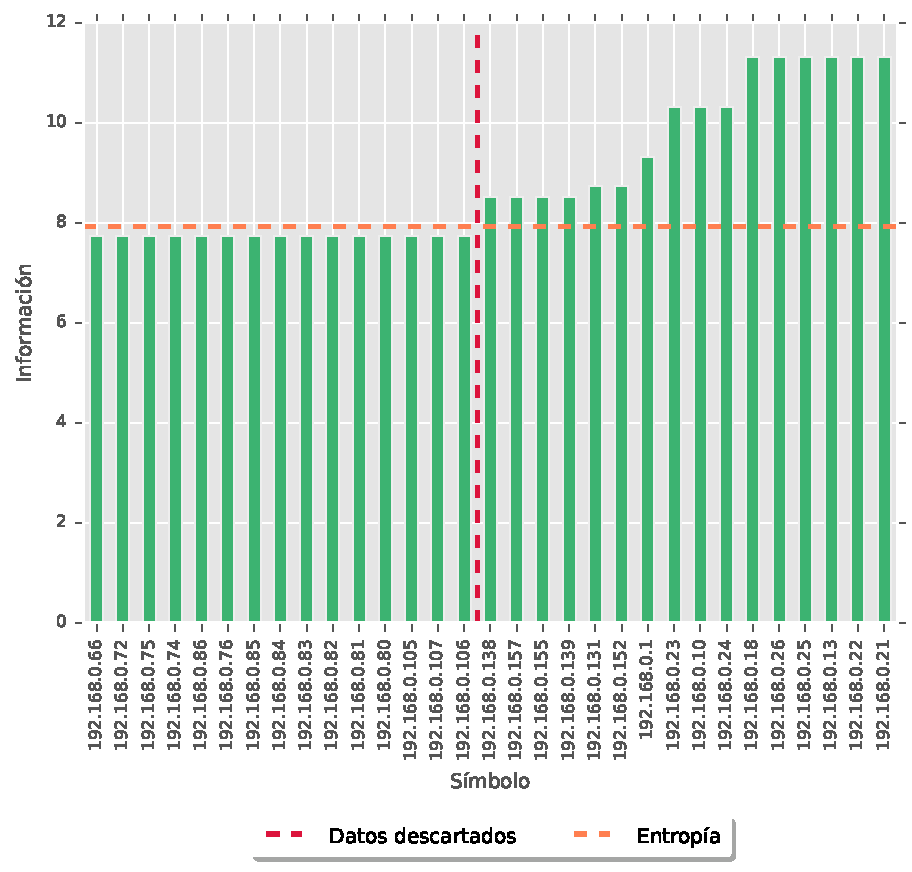
\includegraphics[scale = 0.5]{img/Cumple-information-S1.pdf}
    \caption{Información de los simbolos de la fuente S1 para Cumpleaños}
    \label{informacion_cumple}
  \end{center}
\end{figure}

Esta red presentó pocas \textit{MACs} pero muchas direcciones \textit{IP}.
% Se desconoce la infraestructura de la red como para poder desarrollar conclusiones al respecto de este evento.
Una posible explicación de esta situación podría ser que algún nodo presentó un comportamiento anómalo. Por ejemplo, supongamos que un host envió muchos paquetes a ciertas \textit{IPs} que no estaban en la red, se generaron paquetes \textit{ARP} \textit{who-has} con destino hacia esas \textit{IPs}, entonces como no hubo respuestas esas \textit{IPs} no se agregaron a la tabla, por lo tanto cada vez que el probable nodo anómalo mandaba un paquete hacia algún host que no estaba en la red se generaba un nuevo paquete \textit{ARP}. Por lo tanto si las \textit{IPs} destinos de esos paquetes \textit{ARP} aparecieron muchas veces, su probabilidad sube, su información baja, lo que podría explicar la gran cantidad de nodos distinguidos.